\documentclass[tikz,border=1cm]{standalone}
\begin{document}
    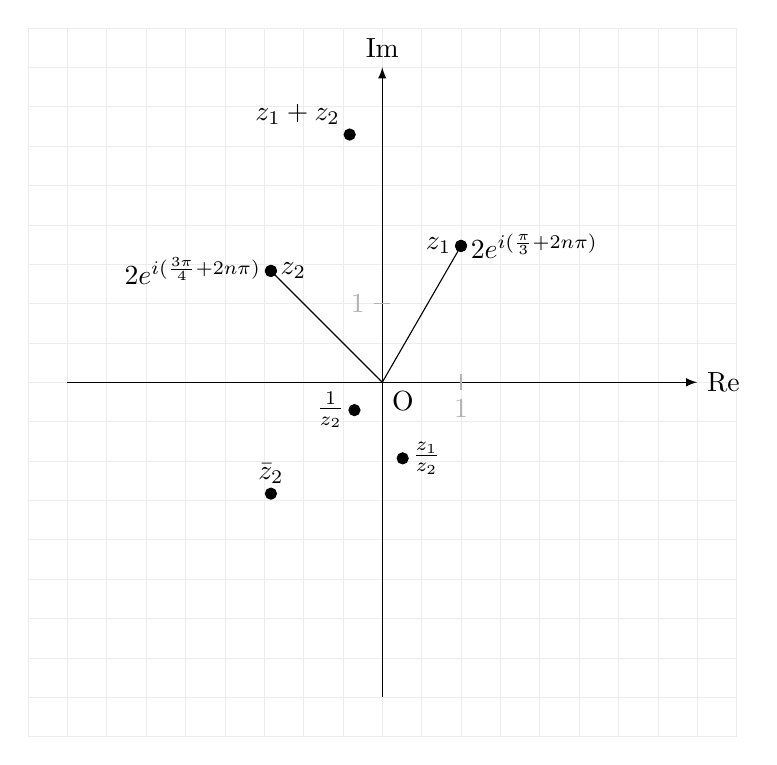
\begin{tikzpicture}
        \draw[very thin,color=gray!15,step=.5] (-4.5,-4.5) grid (4.5,4.5);
        \draw[-latex] (-4,0) -- (4,0) node[right] {Re};
        \draw[-latex] (0,-4) -- (0,4) node[above] {Im};
        \coordinate [label=below right:O] (a) at (0,0);
        \foreach \i in {1}
        \draw[gray!60] (\i,.1)--(\i,-.1) node[below] {$\i$};
        \foreach \i in {1}
        \draw[gray!60] (.1,\i)--(-.1,\i) node[left] {$\i$};

        \filldraw[black,opacity=1] (1, 1.73205) circle(2pt) node[left] {$z_1$};
        \filldraw[black,opacity=1] (-1.414213, 1.414213) circle(2pt) node[right] {$z_2$};
        \filldraw[black,opacity=1] (1 - 1.414213, 1.73205 + 1.414213) circle(2pt) node[above left] {$z_1+z_2$};
        \filldraw[black,opacity=1] (-1.414213, -1.414213) circle(2pt) node[above] {$\bar z_2$};
        \filldraw[black,opacity=1] (-1.414213/4, -1.414213/4) circle(2pt) node[left] {$\frac{1}{z_2}$};
        \filldraw[black,opacity=1] (1, 1.73205) circle(2pt) node[right] {$2e^{i(\frac{\pi}{3} + 2n\pi)}$};
        \filldraw[black,opacity=1] (-1.414213, 1.414213) circle(2pt) node[left] {$2e^{i(\frac{3\pi}{4} + 2n\pi)}$};
        \filldraw[black,opacity=1] (2.44948/4 - 1.414213/4, -2.44948/4-1.414213/4) circle(2pt) node[right] {$\frac{z_1}{z_2}$};

        \draw[black, thin] (0,0) --  (1, 1.73205);
        \draw[black, thin] (0,0) -- (-1.414213, 1.414213);


    \end{tikzpicture}

\end{document}